% NIME Music and Workshop Proceedings Template

% Modified November 2024 by Charles Martin
% Modified December 2019 by Joe Wright
% Created August 2019 by Niccolo Granieri

\documentclass[acmsmall]{nimeart}

%% Rights management information.  This information is sent to you
%% when you complete the rights form.  These commands have SAMPLE
%% values in them; it is your responsibility as an author to replace
%% the commands and values with those provided to you when you
%% complete the rights form.
\setcopyright{cc}
\copyrightyear{2025}
\acmYear{2025}
\acmDOI{}
%% These commands are for a PROCEEDINGS abstract or paper.
%% Make sure this is up to date with the correct edition of NIME.
\acmConference[NIME '25]{International Conference on New Interfaces for Musical Expression}{June 24--27,
  2025}{Canberra, Australia}
%% This suppresses the ACM Reference Format printing.
\settopmatter{printacmref=false}
%%
%%  Uncomment \acmBooktitle if the title of the proceedings is different
%%  from ``Proceedings of ...''!
%%
%%\acmBooktitle{Woodstock '18: ACM Symposium on Neural Gaze Detection,
%%  June 03--05, 2018, Woodstock, NY}
\acmISBN{}


%%
%% end of the preamble, start of the body of the document source.
\begin{document}

%%
%% The "title" command has an optional parameter,
%% allowing the author to define a "short title" to be used in page headers.
\title{The NIME of the Title Is Hope}

% Author information, leave this blank for the initial submission.
\author{Author One}
\affiliation{%
  \institution{Affilitation}
  \city{City}
  \country{Country}
}

\author{Author Two}
\affiliation{%
  \institution{Another Affilitation}
  \city{City}
  \country{Country}
}

\author{Author Three}
\affiliation{%
  \institution{More Affilitations}
  \city{City}
  \country{Country}
}

%%
%% By default, the full list of authors will be used in the page
%% headers. Often, this list is too long, and will overlap
%% other information printed in the page headers. This command allows
%% the author to define a more concise list
%% of authors' names for this purpose.
\renewcommand{\shortauthors}{Trovato et al.}

%%
%% The abstract is a short summary of the work to be presented in the
%% article.
\begin{abstract}
  A clear and well-documented \LaTeX\ document is presented as an
  article formatted for publication by ACM in a conference proceedings
  or journal publication. This uses ``nimeart'', a fork of the ``acmart''
  documentclass with additions for the NIME conference. This
  article presents and explains many of the common variations, as well
  as many of the formatting elements an author may use in the
  preparation of the documentation of their work.
\end{abstract}

%%
%% Keywords. The author(s) should pick words that accurately describe
%% the work being presented. Separate the keywords with commas.
\keywords{Do, Not, Us, This, Code, Put, the, Correct, Terms, for,
  Your, Paper}

%%
%% This command processes the author and affiliation and title
%% information and builds the first part of the formatted document.
\maketitle

\section{Program Notes}

Lorem ipsum dolor sit amet, consectetur adipiscing elit. Duis sodales nunc vitae arcu mattis elementum. Praesent neque arcu, tincidunt a blandit ut, molestie vel massa. In vitae augue mollis, venenatis tellus a, lobortis ex. Aliquam erat volutpat. Suspendisse potenti. Nunc faucibus lacus ut est elementum pharetra. Sed lorem quam, tempus at interdum sit amet, bibendum ut sem. Ut at neque non velit fermentum laoreet. Vivamus ut aliquet velit. Nam id nunc id ante semper dignissim eget eget risus. Nullam suscipit malesuada ante in lobortis.

Plus, some citations to articles: \cite{doe2023,
wizard2022, alien2024}.

\begin{figure}[h]
  \centering
  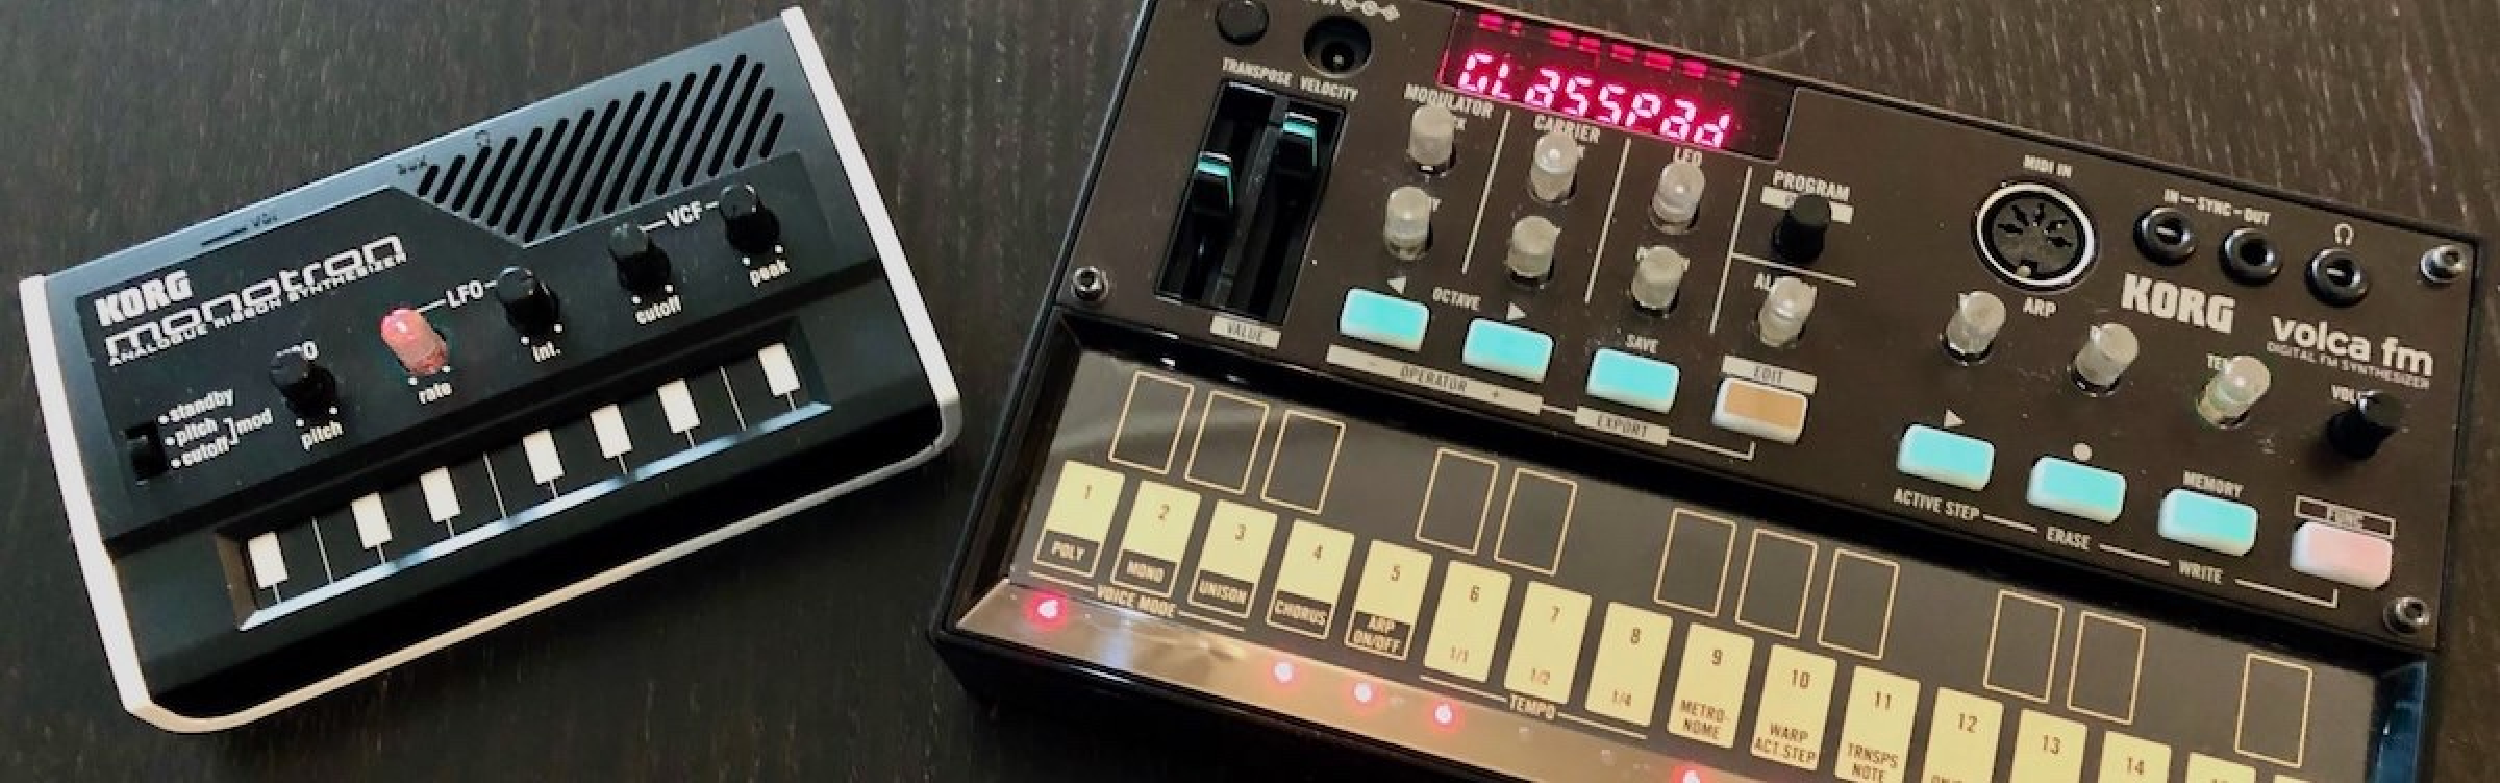
\includegraphics[width=\linewidth]{images/sampleteaser.pdf}
  \caption{Two synthesisers on a table, 2019.}
  \Description{Enjoying looking at two synthesisers.
  A Korg Monotron and a Korg Volca FM.}
\end{figure}

\section{Project Description}

Suspendisse vel pharetra nibh, vel luctus metus. Donec porta dapibus lacinia. Etiam in accumsan enim. Nam vel fermentum libero. Vivamus placerat enim ac sem pharetra cursus. Fusce cursus diam at lacus mattis condimentum. Vestibulum eleifend ante ut ultrices semper. Suspendisse at magna in eros sollicitudin hendrerit eu sed nibh. Integer dapibus felis finibus ornare dignissim. Aliquam semper urna ut purus feugiat vestibulum. In vel nulla volutpat, posuere erat quis, pretium felis. Ut nec tincidunt metus. Fusce libero nunc, mattis vel dignissim non, tempus dapibus nunc. Aliquam enim velit, sagittis non nulla ac, dictum porttitor sapien. Aenean ut volutpat nibh, et porta mi.

Vivamus non purus libero. Orci varius natoque penatibus et magnis dis parturient montes, nascetur ridiculus mus. Nulla a ornare nulla. Proin in convallis libero. Cras ornare pharetra neque quis ultrices. Integer egestas odio convallis orci aliquam, quis tincidunt leo luctus. Duis fringilla leo eget ante ultricies viverra. Quisque elit lacus, egestas vel ultricies quis, eleifend vel purus. Duis eu finibus ex, eu mattis lectus. Duis a laoreet tellus, sed eleifend augue. Sed elementum sem at sapien pellentesque, sit amet varius sapien eleifend. Curabitur ultricies lorem nec dolor ornare, id sodales sapien rutrum.

\section{Technical Notes}

Nulla id dapibus nibh. Suspendisse ultrices dapibus egestas. Sed diam turpis, gravida vitae nibh in, tincidunt hendrerit nulla. Curabitur viverra nibh id lectus volutpat posuere. Fusce tristique condimentum eros, sed mollis ligula euismod sit amet. Proin consectetur dignissim metus, viverra blandit mauris lacinia vel. Vivamus maximus sed elit eu elementum. Nam iaculis vel est vel semper. Nullam pharetra, augue iaculis luctus elementum, urna odio gravida elit, in sagittis ligula magna ac erat.

Suspendisse vel nisl porta, venenatis dui interdum, faucibus risus. Donec congue, dolor quis consequat facilisis, tellus neque lobortis dolor, ullamcorper suscipit turpis massa vitae mauris. Aliquam venenatis augue posuere, pretium turpis dictum, consequat metus. Aenean quis eros enim. Aenean ac magna porttitor, lacinia enim id, facilisis arcu. Donec eleifend mi nec ipsum ultrices posuere. Quisque eu erat venenatis velit dapibus auctor in non ligula. Vestibulum nisl justo, aliquet ut elit a, bibendum pulvinar lectus.

\section{Media Links}

In this section, please provide a list of links to media representations of your submission.

\begin{itemize}
	\item Video: \url{https://www.yournimevideolink.com/younameit}
	\item Audio: \url{https://www.yournimeaudiolink.com/younameit}
\end{itemize}

\section{Ethical Standards}

Please note that an Ethical Standards section is required for all NIME submissions.

This could include information regarding sources of funding, sustainability factors, potential conflicts of interest,  informed consent if the research involved human participants, statement on welfare of animals if the research involved animals, or other ethical factors that are relevant to the work.

% The acknowledgements section is optional and can be removed if not needed.
\begin{acks}
The authors would like to thank\ldots
\\
This work was supported by\ldots
\end{acks}

%%
%% The next two lines define the bibliography style to be used, and
%% the bibliography file.
\bibliographystyle{ACM-Reference-Format}
\bibliography{sample-references}

\end{document}
